\documentclass[tikz,margin=10pt]{standalone}
\usepackage[utf8]{inputenc}
\usepackage[T1]{fontenc}

\usepackage{tikz}
\usepackage{helvet}
\usepackage{amsmath}

\renewcommand\familydefault\sfdefault
\usetikzlibrary{calc}

\usepackage{pgfplots, pgfplotstable}
\pgfplotsset{compat=1.18}

\usetikzlibrary{
	hobby,
	babel,
	intersections,
	spath3,
	shapes.arrows,
	shapes.geometric,
	shapes.symbols,
	fit,
	backgrounds, 
	calc,
	tikzmark,
	decorations.pathreplacing,
	angles,
	arrows.meta,
	quotes,
	positioning,
}


\makeatletter
\long\def\ifnodedefined#1#2#3{%
    \@ifundefined{pgf@sh@ns@#1}{#3}{#2}%
}

\pgfplotsset{
    discontinuous/.style={
    const plot,
    mark=none
   }
}
\makeatother

\begin{document}

{\centering
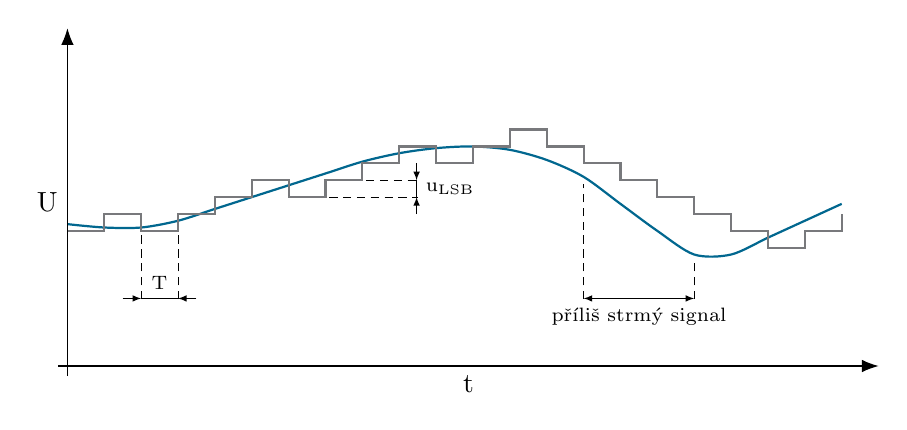
\begin{tikzpicture} [
	helper line/.style = {draw=black, ultra thin, densely dashed, mark=none},
	dim line/.style = {ultra thin, -latex, color=black},
	dim seg/.style = {ultra thin, color=black},
]

\definecolor{themeBlue}{RGB}{1, 103, 143}
\definecolor{themeOrange}{RGB}{221, 109, 16}
\definecolor{themeTeal}{RGB}{18, 54, 69}
\definecolor{themeGrey}{RGB}{120, 121, 124}

\begin{axis}[
	no markers,
    enlargelimits=false, clip=false, axis on top,
    axis lines*=middle,
    axis line style={->, -{Latex[scale=1.25]}},
    %y post scale=.8,
    ytick=\empty, xtick=\empty,
	width=12cm,
	height=6cm,
	legend style={draw=none},
    jump mark left,
    ymin=-.15,ymax=5,
    xmin=-.25, xmax=22,
    xlabel={$ \text{t} $},
  	ylabel={$ \text{U} $},
	ylabel style={rotate=-90},
    every axis plot/.style={thick},
    discontinuous,
    table/create on use/cumulative distribution/.style={
        create col/expr={\pgfmathaccuma + \thisrow{shift}}   
    }
]
\addplot [themeBlue, smooth] table [y=cumulative distribution] {
x	shift
0	2.1
1	-.05
2	0
3	.1
4	.175
5	.175
6	.175
7	.175
8	.175
9	.125
10	.075
11	.025
12 	-.05
13	-.15
14	-.25
15 	-.4
16	-.40
17	-.35
18	0
19	.25
20	.25
21	.25
};

\addplot [themeGrey] table [y=cumulative distribution] {
x shift
0 2
1 .25
2 -.25
3 .25
4 .25
5 .25
6 -.25
7 .25
8 .25
9 .25
10 -.25
11 .25
12 .25
13 -.25
14 -.25
15 -.25
16 -.25
17 -.25
18 -.25
19 -.25
20 .25
21 .25
};

\addplot [helper line] coordinates {(2, .99) (2, 1.97)};
\addplot [helper line] coordinates {(3, .99) (3, 1.97)};

\addplot [dim line] (1.5,1) -- (2,1);
\addplot [dim line] (3.5,1) -- (3,1);
\addplot [dim seg] (2,1) -- (3,1) node[above, sloped, pos = .5, font=\scriptsize] {T};

\addplot [helper line] coordinates {(7.1, 2.5) (9.5, 2.5)};
\addplot [helper line] coordinates {(8.1, 2.75) (9.5, 2.75)};

\addplot [dim line] (9.47, 3) -- (9.47, 2.75);
\addplot [dim line] (9.47, 2.25) -- (9.47, 2.5);
\addplot [dim seg] (9.47, 2.5) -- (9.47, 2.75) node[below, rotate=-90, anchor=west, sloped, pos = .5, font=\scriptsize] {$ \text{u}_{\text{LSB}} $};

\addplot [helper line] coordinates {(14, .99) (14, 2.7)};
\addplot [helper line] coordinates {(17, .99) (17, 1.6)};
\addplot [dim line] (15.5, 1) -- (17, 1);
\addplot [dim line] (15.5, 1) -- (14, 1) node[below, sloped, pos = 0, font=\scriptsize] {příliš strmý signal};

\end{axis}
% 11 -- midpoint
\end{tikzpicture}
\par}
\end{document}